\vspace*{1.5pc}


%%%%%%%%%%%%%%%%%%%%%%%%%%%%%%
\subsection{Methodology}
%%%%%%%%%%%%%%%%%%%%%%%%%%%%%%
\label{sec:methodology}

\begin{figure}
\centering
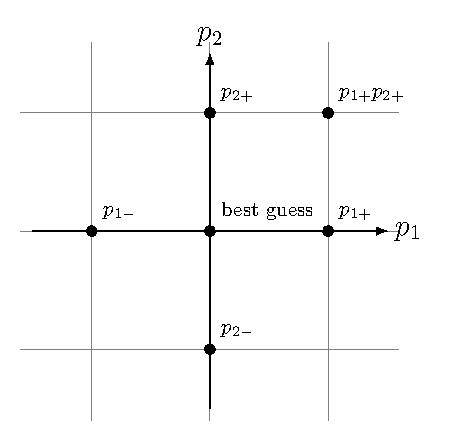
\includegraphics[width=.5\linewidth]{Dari/simulation_grid.pdf}
\caption{Illustration of the required grid for a second-order Taylor expansion in a
two-dimensional parameter space.}\label{fig:grid}
\end{figure}

We evaluate the variations of the flux power spectrum with our standard set of parameters $\vec{x}$
%\begin{equation}
%\vec{x} =  \left(m_\nu^{\mathrm{eff}}, h, \: \Omega_m, \: n_s, \: \sigma_8, \: T_0^{z=3}, \: \gamma^{z=3}, \: %A^\tau, \: \eta^\tau \right)^T
%\end{equation}
around our central (herein \emph{best guess}) model $\vec{x}_0$ using a second-order Taylor expansion:\\
\begin{align}
\label{eq:Taylor}
f(\vec{x}_0 + \Delta \vec{x}) &\simeq f(\vec{x}_0)\\
&+ \sum_i \left. \cfrac{\partial f}{\partial x_i} \right\vert_{\vec{x} = \vec{x}_0} \Delta x_i \\
&+ \frac{1}{2}  \sum_{i} \sum_{j}  \left. \cfrac{\partial^2 f}{\partial x_i \partial x_j} \right\vert_{\vec{x} = \vec{x}_0} \Delta x_i \Delta x_j \\
&+ \mathcal{O} \left( \left\vert \Delta \vec{x} \right\vert^3 \right) 
\end{align} \\

In addition to our central model $\vec{x}_0$, each parameter $x_i$ in our simulation grid requires running $2n$ additional simulations for the $\pm \Delta x_i$ first-order terms (second row of Eq.~\ref{eq:Taylor}) and $n \left( n-1 \right) / 2$ simulations for the second-order cross-terms (third row of Eq.~\ref{eq:Taylor}), where $n$ is the number of parameters. With this lattice, all derivatives are approximated  to second order except the
cross derivatives which are approximated to first order. This approximation is justified by the fact that the parameters are reasonably decoupled, and it allowed us to reduce the CPU time consumption since second-order cross derivatives would require additional $n(n-1)/2$ simulations. The parameters at hand, \textit{i.e.} the components of $\vec{x}$, are of three categories which I describe promptly below. Their central and step values are recaped in Tab.~\ref{tab:parameter_values}.

\begin{table}
\begin{center}
\begin{tabular}{ccccl}
\hline \\[-10pt]
\hline \\[-10pt]
\textbf{parameter} &  & $\pmb{x_{0,i}}$ & & $\pmb{\Delta x_i}$ \\[2pt]
\hline \\[-10pt]
\hline \\[-10pt]
\multicolumn{5}{l}{\textbf{cosmological}} \\[2pt]
$h$ & $=$ & $0.675$ & $\pm$ & $0.05$  \\[2pt]
$\Omega_m$ & $=$ & $0.31$ & $\pm$ & $0.05$  \\[2pt]
$\sigma_8$ & $=$ & $0.83$ & $\pm$ & $0.05$  \\[2pt]
$n_s$ & $=$ & $0.96$ & $\pm$ & $0.05$  \\[2pt]
\hline \\[-10pt]
\multicolumn{5}{l}{\textbf{non-$\Lambda$CDM / neutrino}} \\[2pt]
$d n_s / d \ln k$ & $=$ & $0.00$ & $\pm$ & $0.02$  \\[2pt]
$N_{\mathrm{eff}}$ & $=$ & $3.046$ & $\pm$ & $1.000$  \\[2pt]
$\sum m_\nu / \mathrm{eV}$ & $=$ & $0.0$ & $+$ & $0.4,0.8$  \\[2pt]
$\mathrm{keV}/m_x$ & $=$ & $0.0$ & $+$ & $0.2,0.4$  \\[2pt]
\hline \\[-10pt]
\multicolumn{5}{l}{\textbf{astrophysical}} \\[2pt]
$T^{z=3}_0/10^3\mathrm{K}$ & $=$ & $14.0$ & $\pm$ & $7.0$  \\[2pt]
$\gamma^{z=3}$ & $=$ & $1.3$ & $\pm$ & $0.3$  \\[2pt]
$A^\tau / 10^{-3}$ & $=$ & $2.5$ & $\pm$ & $2.0$  \\[2pt]
$\eta^\tau$ & $=$ & $3.7$ & $\pm$ & $0.4$  \\[2pt]
$z_\star$ & $=$ & $12.0$ & $\pm$ & $4.0$  \\[2pt]
\hline \\[-10pt]
\end{tabular}
\end{center}
\caption{central (middle row) and step (right-most row) values of each parameter in our Taylor grid.}
\label{tab:parameter_values}
\end{table}



\subsubsection{Cosmological Parameters}
\label{sec:cosmo_param}

We investigate the impact on the flux power spectrum of four cosmological parameters based on the central values and $68\%$ CL bounds from the Planck collaboration best fit: \\
\begin{itemize}
\item[$\bullet$] the current expansion rate $H_0$ in units of $100~h~\mathrm{km}~s^{-1}\mathrm{Mpc}^{-1}$;\\
\item[$\bullet$] the total (baryon + neutrino + dark) matter density $\Omega_m$ in units of critical energy density; \\
\item[$\bullet$] $\sigma_8$, the variance in the matter density fluctuations at $8 h^{-1}\mathrm{Mpc}$ (see Eq.~\ref{def:sig8});\\
\item[$\bullet$] the spectral index $n_s \doteq \left.\cfrac{d P_s}{d \ln k}\right\vert_{k=k_\star}$ of the primordial power spectrum of scalar modes of perturbations.\\
\end{itemize}

We chose the range of variation for these parameters so as to include other recent constraints from the Wilkinson Microwave
Anisotropy Probe seven years data \citep{Komatsu2011}, the South Pole Telescope data \citep{Hou2012} and the SuperNova Legacy Survey
three year data \citep{Conley2011, Sullivan2011}, thus taking into account the fact that results from Planck for $H_0$ (\textit{resp.}
$\Omega_m$) are low (\textit{resp.} high) compared to other measurements. Central values at redshift $z=0$ and step range for each of the cosmological parameters are given in the first tier of Tab.~\ref{tab:parameter_values}.  

\begin{figure}
\begin{center}
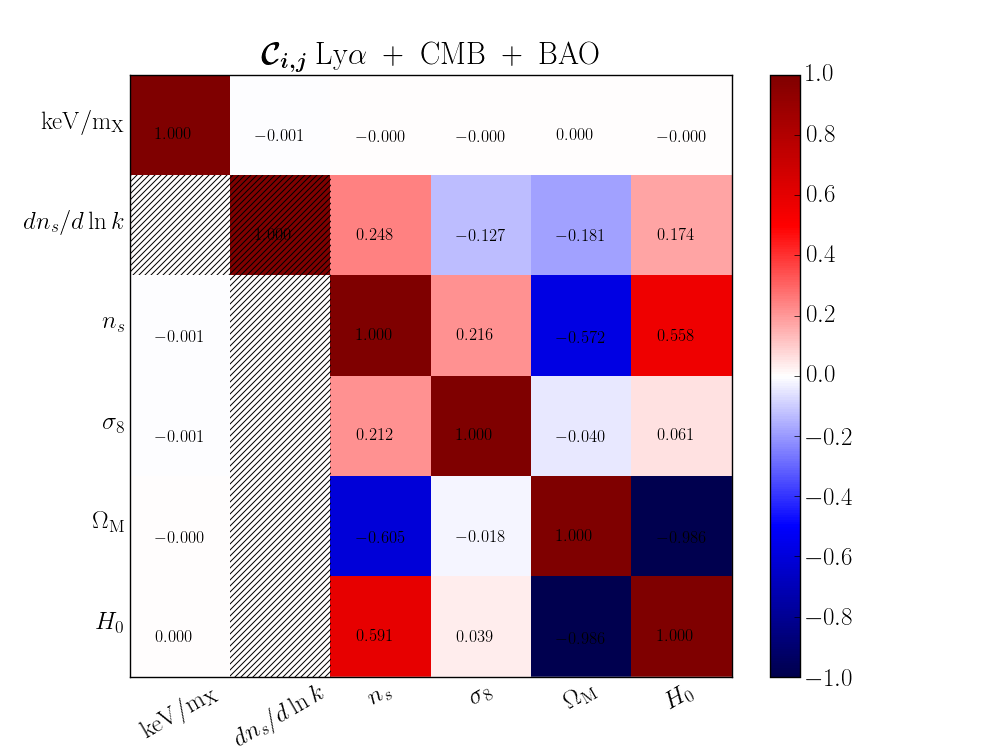
\includegraphics[width=0.9\columnwidth]{Covariance/WDM_CORR_Lya+CMB+BAO_COSMO.png}
\caption{Correlation matrix of the cosmological parameters, spectral index running, and thermal relic dark matter mass using Ly-$\alpha$ + $H_0$ + CMB + BAO data set (see Sec.~\ref{sec:data} for definition), with free (top right triangle) and fixed (bottom left triangle) running in our likelihood analysis.}
\label{fig:C_cosmo}
\end{center}
\end{figure}


\subsubsection{Astrophysical Parameters}
\label{sec:astro_param}

We also investigate the impact on the flux power spectrum of five astrophysical parameters controlling the IGM thermal state and re-ionization history: \\
\begin{itemize}
\item[$\bullet$] $T^{z=3}_0 \doteq T(\delta=0, z=3)$ the mean IGM temperature at $z=3$ (see Eq.~\ref{eq:IGM});\\
\item[$\bullet$] $\gamma(z=3)$ the IGM temperature density index at $z=3$ (see Eq.~\ref{eq:IGM});\\
\item[$\bullet$] $A^\tau \doteq \tau_{\mathrm{eff}}(z=0)$ the effective Ly-$\alpha$ optical depth at $z=3$ (see Eq.~\ref{eq:optdepth});\\
\item[$\bullet$] $\eta^\tau \doteq \left. \cfrac{d \tau_{\mathrm{eff}}}{d \ln z} \right\vert_{z=3}$ the effective Ly-$\alpha$ optical depth redshift index at $z=3$ (see Eq.~\ref{eq:optdepth}); \\
\item[$\bullet$] $z_\star$ the redshift where reionization fraction is $50\%$. \\
\end{itemize} 

As introduced in Sec.~\ref{sec:pipeline}, the relationship between the mean temperature of the IGM and the matter density is explicited in Eq.~\ref{eq:IGM}. For a given simulation, we measure $T_0^{z=3}$ and $\gamma^{z=3}$ by building, for each redshift $z$, the $ T- \rho$ diagram from our sample of $10^6$ particles, shown in Fig.~\ref{fig:rhotemp}. In the low density and low temperature region where the IGM lies, a linear fit of $\ln(T)$ as a function of $\ln(\delta)$ allow us to determine $T_0(z)$ and $\gamma(z)$. The parameter $\gamma(z)$  is monotonically and smoothly decreasing with redshift,  whereas  $T_0(z)$  presents two regimes with a break at $z\sim 3$. The latter distribution follows notably well the measurements of \cite{Becker2011}. As a consequence, in \cite{Palanque2015a}, we fixed the redshift dependences to those measured in the simulations, and we let free two global parameters $T_0$ and $\gamma$. \\

Currently, we release the shapes of $T_0(z)$ and $\gamma(z)$ whose evolution with redshift we model by power laws:\\

\begin{equation}
\label{eq:IGM_new_model}
\begin{array}{c}
T_0(z) = T_0^{z=3} \left( \cfrac{1+z}{4} \right)^{\eta^T} \\
\\
\gamma (z) = \gamma^{z=3} \left( \cfrac{1+z}{4} \right)^{\eta^\gamma}
\end{array}
\end{equation}\\

This model no longer requires one but two parameters to describe $\gamma$: its value and its redshift index at $z=3$: 
\begin{equation}
\eta^\gamma = \left. \frac{d \gamma}{d \ln z} \right\vert_{z=3}
\end{equation}
For the mean IGM temperature at $\rho = \bar{\rho}$, it requires three parameters instead of one: its value at $z=3$ as well as its redshift index below and above a break at $z=3$: 
\begin{equation}
\eta^{T}_{\pm} \doteq \left. \frac{d T_0}{d \ln z} \right\vert_{z \lessgtr 3} 
\end{equation}

In summary, we use five parameters to model the IGM temperature: $T_0^{z=3}$, $\eta^{T}_{-}$, $\eta^{T}_{+}$, $\gamma^{z=3}$ and $\eta^\gamma$ which we float in our fit procedure and constrain using our particle sample of our hydrodynamics simulations. As explained in Sec.~\ref{sec:particle_sample}, we only require $\left( \texttt{AMPL}, \texttt{GRAD} \right)$ as input for our simulations, which have the direct correspondance with the quoted values of $\left( T_0^{z=3}, \gamma^{z=3} \right)$ in Tab.~\ref{tab:parameter_values}. The following two parameters, $A^\tau$ and $\eta^\tau$, introduced in Eq.~\ref{eq:optdepth}, serve as renormalizing paramaters of the Ly-$\alpha$ effective optical depth derived in each pixel of the LOS sample I trace. Therefore there is no need to run the SPH+$N$body part of the pipeline when computing the terms with these parameters off from their central values.\\

\begin{figure}
\begin{center}
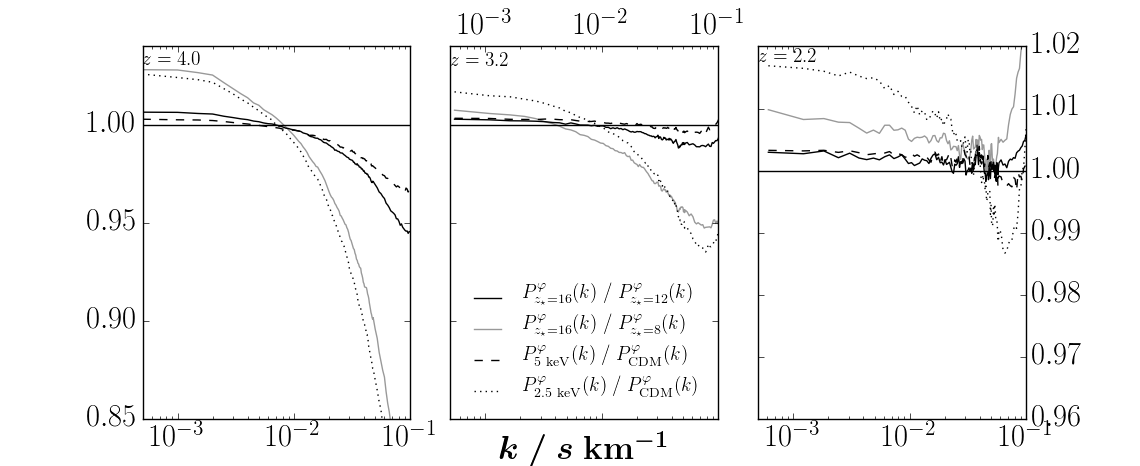
\includegraphics[width=\columnwidth]{Reio/zreio08091516.png}
\caption{1D Ly-$\alpha$ power spectra at redshifts $z=4.0, 3.2$ and $2.2$ normalized to the benchmark central model $P^\varphi_{\mathrm{cdm}} (k) = P^\varphi_{z_\star = 12} (k)$ with the exception of the solid black line which is normalised to the more realistic $z_\star = 8$.}
\label{fig:zreio_flux}
\end{center}
\end{figure}

Finally, the hydrogen reionisation history will alter the pressure 
smoothing scale of the IGM gas, particularly at redshifts approaching the 
tail-end of the reionisation at $z \sim 6-8$ \citep{Gnedin1998}. The effect of the redshift to reionization $z_\star$ on the flux power spectrum is quasi-degenerate with the effect of free-streaming of thermal dark matter relics of mass $m_x = 2.5$ and $5$ keV, used in our grid of simulations, as is apparent on Fig.~\ref{fig:zreio_flux}. Our central model is centered on $z_\star = 12$, which is nowadays considered to be an unrealistically large value. In a first approach, I run the complete hydrodynamic simulations which have a reionization redshift steps of $\Delta z_\star = \pm 4$, and construct the flux power spectrum for all the first and second order terms in the Taylor expansion. We must account for the degenerate effect of reionization redshift --- especially for the pure WDM and C+WDM studies --- and to do so requires modeling the evolution of the flux power spectrum with $z_\star$. In a second approach, I computed, in addition to the $z_\star = 12$ central model, the flux power spectra with $z_\star = 8, 9, 15$ and $16$, and use them to build a systematic nuissance parameter which accounts for the reionization redshift which I later describe in Sec.~\ref{sec:fit_igm}.

\subsubsection{non-$\Lambda$CDM and Neutrino Parameters}
\label{sec:ncdm_param}

We investigate the impact of massive active neutrinos as C+HDM (\textit{a.k.a.} $\Lambda$CDM$\nu$) on the flux power spectrum by running $\sum m_\nu$ as simulation parameter. Our best guess central model is centered on a neutrinoless pure CDM flat Universe ($\sum m_\nu = 0$). Neutrino masses must be strictly positive. Therefore the first-order terms in the Taylor expansion are computed with $\sum m_\nu = 0.4~\mathrm{eV}$, while the cross terms are computed with $\sum m_\nu = 0.8~\mathrm{eV}$. \\

To investigate the mass of sterile neutrinos $m_{\nu_s}$ or thermal relics $m_x$ as pure warm dark matter, the relevant parameter is the inverse of mass (which is proportional to the thermal velocity, or the free-streaming length). The mass mapping between both models can be used as a bijection to enable us to directly convert our bounds on $m_x$ into bounds on $m^{\mathrm{nrp}}_{\nu_s}$ without the need to run additional simulations. The \emph{best guess} configuration is at $\mathrm{keV}/m_x = 0$, and since masses must be positive, the first order and cross terms are computed at $\mathrm{keV}/m_x = 0.2, 0.4$ respectively. \\


I also produced simulations with $N_{\mathrm{eff}} = 3.046 \pm 1.000$ and all the associated cross-terms to investigate whether the 1D Ly-$\alpha$ forest power spectrum can detect evidence of additional thermalized neutrino species (such as the tentative existance of eV scale sterile neutrinos hinted to by reactor experiment anomalies). More realistically, we make use of the computed power spectrum to check for correlations with other cosmological parameters, or a combination of them.\\

Finally, as we pointed out in \cite{Palanque2015b}, our best fit issues a slight inconsistency of $2.3 \sigma$ on the spectral index $n_s$ with respect to the Planck collaboration best fit. It is likely this tension be aliviated through a yet poorly-understood systematic in our Ly-$\alpha$ data. In the off chance that our value holds, it could constitute evidence for non-zero running on the spectral index, $n_{\mathrm{run}} = 2 \times d n_s / d \ln k$, which appears in the first-order expansion of the initial scalar power spectrum
\begin{equation}
\label{eq:PS_nrun}
P_s ~=~ \mathcal{A}_s ~\left( \frac{k}{k_\star} \right)^{n_s + \frac{d n_s}{d \ln k} \ln \left( \frac{k}{k_\star} \right)}
\end{equation} 
where $k_\star = 0.05 ~\mathrm{Mpc}^{-1}$ is the pivot scale of the CMB. To test non-zero $n_{\mathrm{run}}$ models, I produced the flux power spectrum with $d n_s / d \ln k = 0.00 \pm 0.02$ and $\pm 0.04$, with the cross terms computed with the $0.02$ step size. 

\subsubsection{Off-Grid}
\label{sec:offgrid}

In addition to the simulation grid parameters, collected in
\begin{equation}
\vec{x} = \left( m_\nu^{\mathrm{eff}}, h, \Omega_m, \sigma_8, n_s, \frac{d n_s}{d \ln k}, N_{\mathrm{eff}}, z_\star, T_0^{z=3}, \gamma^{z=3}, A^\tau, \eta^\tau \right)^{\mathrm{T}}
\end{equation} where $m_\nu^{\mathrm{eff}} = m^{\mathrm{nrp}}_{\nu_s}$ is the mass of NRP sterile neutrinos as pure warm dark matter particles, and $m_\nu^{\mathrm{eff}} = \sum m_\nu$ is for massive active neutrinos as C+HDM; we also run off-grid simulations where we set $\vec{x} = \vec{x}_0$ for the investigation into C+WDM and RPSN as pure cool dark matter cosmologies. \\

For RPSN models, $m_\nu^{\mathrm{eff}}$ is set to the mass of the keV scale sterile neutrino $m^{\mathrm{rp}}_{\nu_s}$ and the lepton asymmetry parameter that boosts its production at early times $\mathcal{L}_6$ is cast as an additional independant input parameter. The 8 simulations I run with RPSN as pure cool dark matter are:
\begin{equation}
\label{eq:RPSN_models_simu}
\begin{array}{c}
\mathrm{M}3\mathrm{L}16^\star \\
\mathrm{M}4\mathrm{L}12^\star \\
\mathrm{M}6\mathrm{L}6 \\
\mathrm{M}6\mathrm{L}9^\star \\
\mathrm{M}7\mathrm{L}8^\star \\
\mathrm{M}8\mathrm{L}4 \\
\mathrm{M}8\mathrm{L}8^\star \\
\mathrm{M}13\mathrm{L}6^\star
\end{array}
\end{equation} with the nomenclature of M $\equiv m^{\mathrm{rp}}_{\nu_s}$ and L $\equiv \mathcal{L}_6$ and the star superscript denoting a coolest RPSN model for that specific mass.\\


For C+WDM, $m_\nu^{\mathrm{eff}}$ is set to the thermal relic mass $m_x$ (or rather, its inverse so that the best guess model is at $0$) and I input the relative dark matter fraction of the warm component $F_{\mathrm{wdm}}$ as an additional independant parameter. Tab.~\ref{tab:cwdm_grid} recaps the 28 off-grid models for the C+WDM project. No cross-terms are computed for either of C+WDM or RPSN projects. Rather, the constraints are obtained by scanning the $\left( m_{\nu_s}^{\mathrm{rp}}, \mathcal{L}_6 \right)$ and $\left( m^{\mathrm{eff}}_\nu, F_{\mathrm{wdm}} \right)$ parameter spaces.

\begin{table}
\begin{center}
\begin{tabular}{cc}
\hline \\[-10pt]
\textbf{warm component abundance} & \textbf{thermal relic mass} \\[2pt]
$\pmb{F_{\mathrm{wdm}}}$ & $\pmb{\mathrm{keV}/m_x}$ \\[2pt]
\hline \\[-10pt]
$1.00$ & $0.1$ \\[2pt]
 & $0.2$ \\[2pt]
 & $0.3$ \\[2pt]
 & $0.4$ \\[2pt]
 & $0.7$ \\[2pt]
\hline \\[-10pt]
$0.75$ & $0.3$ \\[2pt]
 & $0.4$ \\[2pt]
\hline \\[-10pt]
$0.50$ & $0.1$ \\[2pt]
 & $0.2$ \\[2pt]
 & $0.4$ \\[2pt]
 & $0.7$ \\[2pt]
\hline \\[-10pt]
$0.30$ & $0.05$ \\[2pt]
 & $0.7$ \\[2pt]
 & $1.0$ \\[2pt]
\hline \\[-10pt]
$0.20$ & $0.1$ \\[2pt]
 & $0.2$ \\[2pt]
 & $0.4$ \\[2pt]
 & $1.5$ \\[2pt]
\hline \\[-10pt]
$0.10$ & $0.1$ \\[2pt]
 & $0.2$ \\[2pt]
 & $0.4$ \\[2pt]
 & $0.7$ \\[2pt]
 & $1.0$ \\[2pt]
 & $1.5$ \\[2pt]
\hline \\[-10pt]
$0.05$ & $0.1$ \\[2pt]
 & $0.2$ \\[2pt]
 & $0.3$ \\[2pt] 
 & $0.4$ \\[2pt]
\hline \\[-10pt]
\end{tabular}
\end{center}
\caption{$\left( m_x, F_{\mathrm{wdm}} \right)$ values of our 28 C+WDM models, off-grid from our Taylor expansion. All other parameters are set to their central values in the middle column of Tab.\ref{tab:parameter_values}.}
\label{tab:cwdm_grid}
\end{table}



%%%%%%%%%%%%%%%%%%%%%%%%%%%%%%
\subsection{Fitting Parameters}
%%%%%%%%%%%%%%%%%%%%%%%%%%%%%%

Ensuing the complete simulation pipeline illustrated in Fig.~\ref{fig:pipeline}, we have at our hands a set of Ly-$\alpha$ power spectra and IGM temperature - density power laws in 13 redshift bins for each parameter value in Tab.~\ref{tab:parameter_values}, as well as the ones listed in Tab.~\ref{tab:cwdm_grid} and Eq.~\ref{eq:RPSN_models_simu} for the C+WDM and RPSN projects exclusively. Our fitting procedure, described in Sec.~\ref{sec:likelihood} below, searches for the optimal values of the parameters just mentionned. In this current section, I go over the set of nuisance parameters which are also fitted in addition to the cosmological, astrophysical and NCDM parameters. There are sub-divided into 3 distinct categories, which I detail in the following subsections.

\subsubsection{IGM Thermal State}
\label{sec:fit_igm}

\begin{figure}
\begin{center}
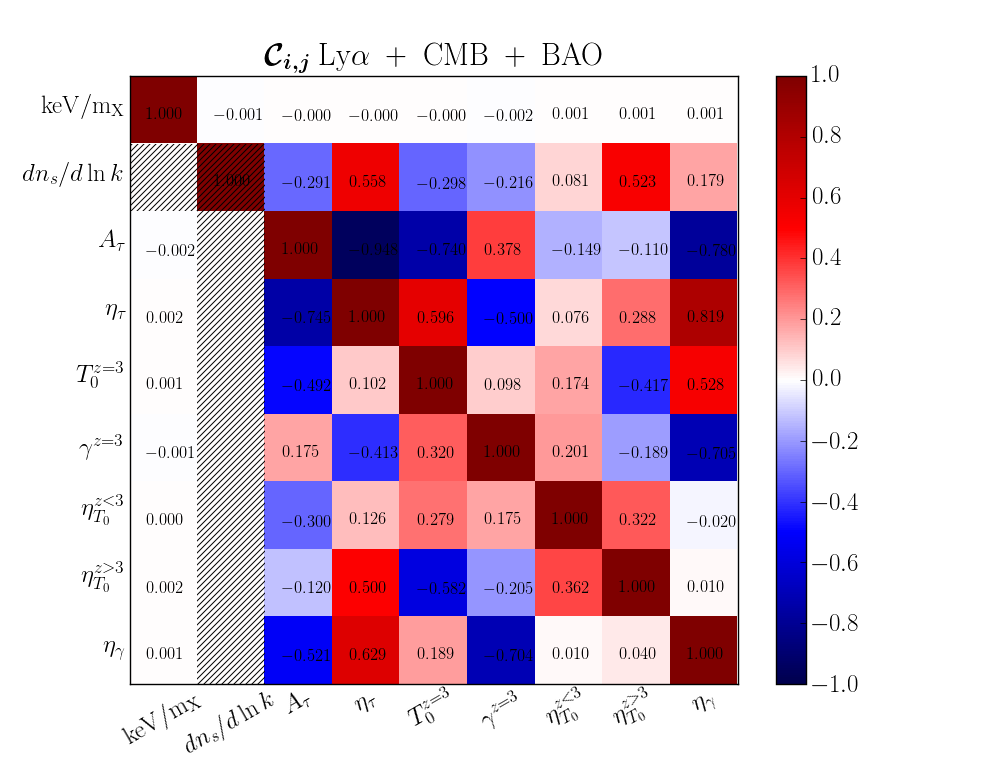
\includegraphics[width=0.9\columnwidth]{Covariance/WDM_CORR_Lya+CMB+BAO_IGM.png}
\caption{Same as Fig.~\ref{fig:C_cosmo} for the astrophysical parameters.}
\label{fig:C_astro}
\end{center}
\end{figure}

As in most optically-thin hydrodynamics simulations, the ionizing (UV) background causes the Hydrogen to quickly become highly ionized. This is qualitatively inaccurate since reionization processes are non-instantaneous and operate inhomogeneously in space due to density contrasts. Although hydrodynamics simulations are required to tackle this shortcoming self-consistently, our study is concerned with modeling the Ly-$\alpha$ forest at $z<5$, well after reionization processes have completed. The redshift at which the UV background onsets, however, affects the Jeans smoothing scale of the baryon gas \citep{Gnedin&Hui98} in a manner similar to the free streaming scale of warm dark matter particles. Altering the reionization redshift $z_{\star}$ impacts the amount of time that gas pressure has to suppress small-scale density fluctuations. It is therefore necessary to explore different thermal histories of the IGM in order to lift the degeneracy between Jeans smoothing scale and WDM free streaming scale. 
Fig.~13 of \citep{McDonald2005} shows that an increase in the redshift of reionization from $z_{\star}=7$ to 17 suppresses the Ly$\alpha$ flux power spectrum in the largest  $k$-modes present in the BOSS data ($k \sim 0.02~s \: \rm{km^{-1}}$) by about 1\% at $z=2.1$ and 4\% at $z=4.0$. Given the reduced range allowed for $z_{\star}$ by recent Planck measurements, these shifts are reduced to percent-level at most. We implement another multiplicative nuisance parameter $\mathcal{C}_\star(k)$ in our likelihood to take into account the effect of $z_{\star}$ on the IGM thermal history. This parameter is given by 
\begin{equation}
\mathcal{C}_\star(k) = \alpha_\star(z) + \beta_\star(z) k+\gamma_\star(z) k^2 \;,
\end{equation}
where $\alpha_\star$, $\beta_\star$, and $\gamma_\star$ are taken from \citep{McDonald2005} and 
interpolated with respect to the central model to our range of  redshift. They are in agreement with the impact of $z_\star$ I derived from the hydrodynamics simulations I ran (after this approach, as a secondary, complementary one).\\

Since the redshift of reionization is  treated as a nuisance parameter in the fit,  we add a $z_{\star} = 9.0 \pm 1.5$ prior  to our likelihood. The central value and range of this prior are defined in order to encompass the most recent measurements of the redshift of reionization: $10.5\pm 1.1$ from WMAP9+BAO+H0~\cite{WMAP9}, $9.9\pm 1.8$ from  Planck TT temperature data at all multipoles and LFI-based polarization data at low ($\ell<30$) multipoles (PlanckTT+`lowP')~\cite{Planck2015}, $10.0\pm 1.7$ when also including the $\ell>30$ HFI polarization data  (PlanckTTEE+`lowP')~\cite{Planck2015}. The latter constraints were revised to $8.11\pm 0.93$ and $8.24\pm0.88$ respectively in the latest incarnation where the `lowP' likelihood was replaced with the `SIMlow' likelihood that includes the HFI-based polarization for $\ell\leq 20$~\cite{Planck2016PolarReio}. Values ranging from 7.8 to 8.8 are  obtained by the Planck collaboration for a given choice of CMB temperature and polarization data set, when varying the model of reionization adopted~\cite{Planck2016Reio}.


\subsubsection{Instrumental Noise}

We model a possible redshift-dependent correction to the spectrograph resolution with the multiplicative factor 
\begin{equation}
\label{eq:Nuis1}
\mathcal{C}_{\mathrm{reso}} = e^{ - \left( \alpha_{\mathrm{reso}} + \beta_{\mathrm{reso}} (z-3) \right) \times k^2}
\end{equation} where $\alpha_{\mathrm{reso}}$ and $\beta_{\mathrm{reso}}$ are allowed to vary around a null value with a Gaussian constraint of $\sigma = \left( 5 \rm{km} s^{-1} \right)^2$. We also quantify the uncertainty in each 12 redshift bins of the data by multiplicative factors $\alpha^{\rm{noise}}_{\langle z \rangle}$ where $\langle z \rangle = 2.2, 2.4, ..., 4.4$. This totals 14 free parameters accounting for data uncertainty and spectrograph resolution in our likelihood.\\

\begin{figure}
\begin{center}
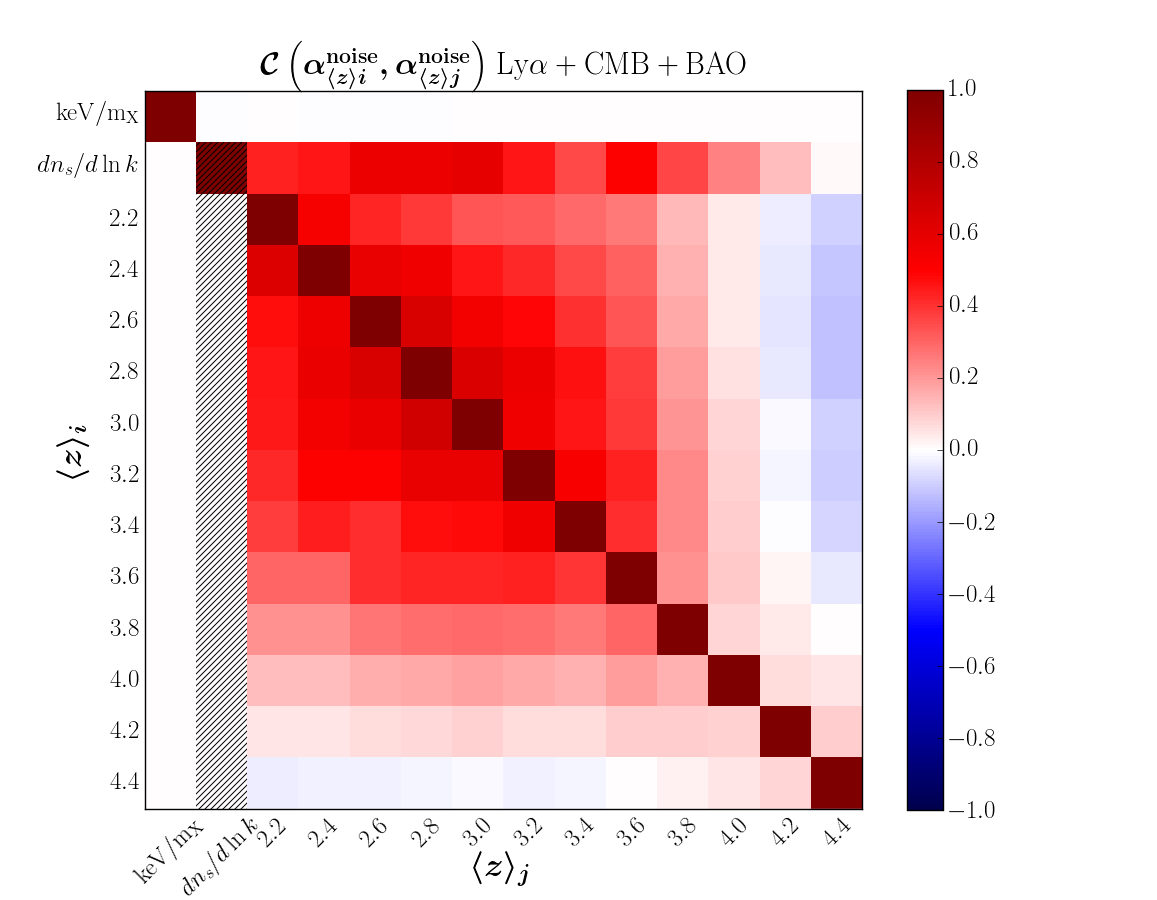
\includegraphics[width=0.9\columnwidth]{Covariance/WDM_CORR_Lya+CMB+BAO_NOISE.png}
\caption{Same as Fig.~\ref{fig:C_cosmo} for the instrument noise parameters}
\label{fig:C_reso}
\end{center}
\end{figure}


\subsubsection{Other Astrophysical Nuisance Parameters}

The hydrodynamics simulations I describe in Sec.~\ref{sec:gadget} are used to compute the 1D Ly-$\alpha$ flux power spectrum from a neutral Hydrogen field. A number of astrophysical feedback processes are poorly quantitatively today and require the addition of systematics. We model the impact of feedbacks from Active Galactic Nuclei (AGN) and Supernov\ae (SN) on the Ly-$\alpha$ transmitted flux by implementing the multiplicative factors
\begin{equation}
\label{eq:Nuis2}
\left\{
\begin{split}
& \mathcal{C}^{\rm{feedback}}_{\rm{AGN}} (k) = \left( \alpha_{\rm{AGN}}(z) + \beta_{\rm{AGN}}(z) \times k \right) \times \alpha^{\rm{feedback}}_{\rm{AGN}} \\
\\
& \mathcal{C}^{\rm{feedback}}_{\rm{SN}} (k) = \left( \alpha_{\rm{SN}}(z) + \beta_{\rm{SN}}(z) \times k \right) \times \alpha^{\rm{feedback}}_{\rm{SN}}
\end{split}
\right.
\end{equation} where the $\alpha_{\rm{AGN, SN}}$ and $\beta_{\rm{AGN, SN}}$ coefficients are derived from \cite{Feedbacks}. An additional parameter is implemented to account for fluctuations in the intensity of the ionizing background, commonly referred to as UV fluctuations. Similar to \cite{UVbackground}, we implement an additive correction proportional to the transmitted flux power spectrum at  pivot point $k_{p} = 0.009 ~s~ \mathrm{km}^{-1}$, $\mathcal{C}_{\rm{UV}}$, which is $k$-independent but evolves with redshift proportionally to the power spectrum. Finally, we account for any damped Lyman-alpha (DLA) systems we might not have removed in our pipeline by introducing a $k$-dependent multiplicative correction (see \cite{McDonald2005} for justification of the analytical form)
\begin{equation}
\label{eq:Nuis3}
\mathcal{C}_{\rm DLA}(k) = \left( \frac{1}{15,000 ~k - 8.9} + 0.018 \right) \times 0.2 \times \alpha_{\rm{DLA}}
\end{equation} where $\alpha_{\rm{DLA}}$ is free to vary in the likelihood fit. 

\begin{figure}
\begin{center}
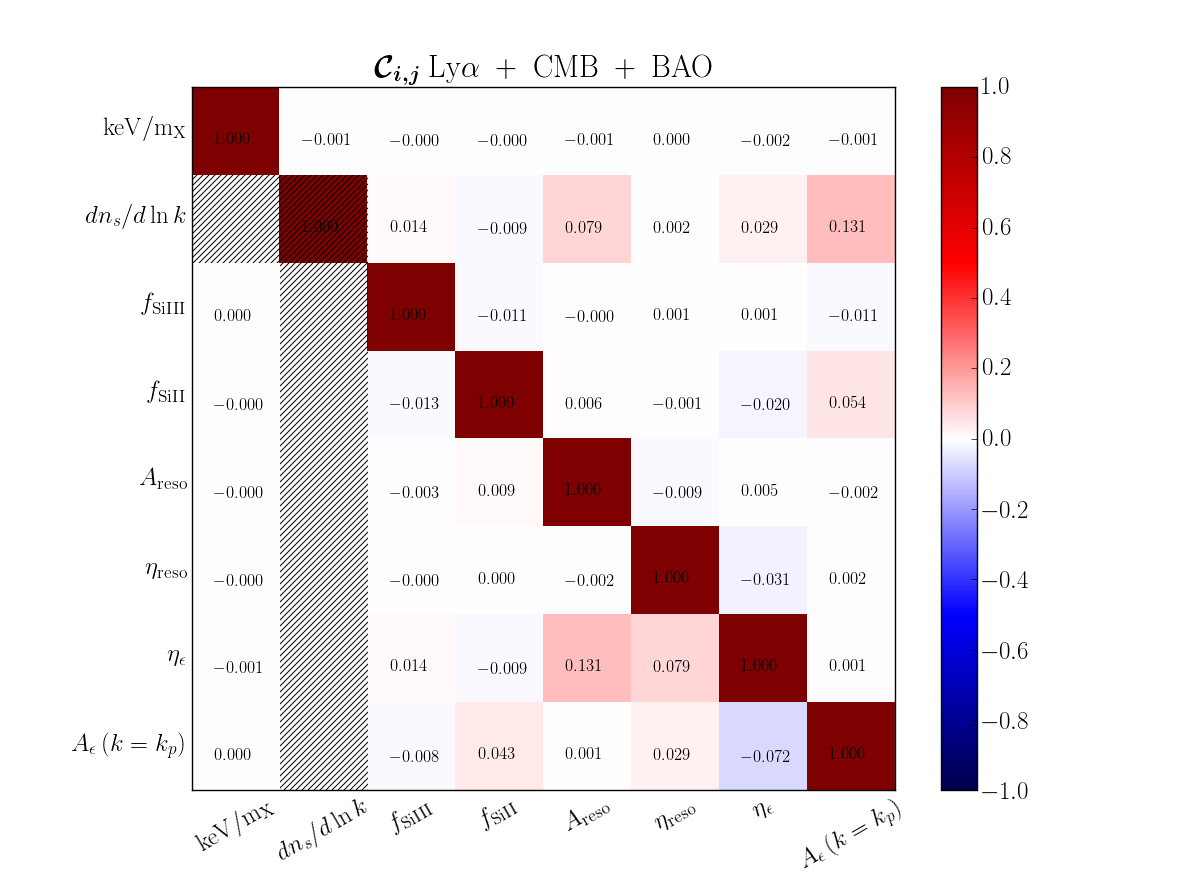
\includegraphics[width=0.9\columnwidth]{Covariance/WDM_CORR_Lya+CMB+BAO_NUIS.png}
\caption{Same as Fig.~\ref{fig:C_cosmo} for our set of additional nuisance parameters.}
\label{fig:C_nuis}
\end{center}
\end{figure}


%%%%%%%%%%%%%%%%%%%%%%%%%%%%%%
\subsection{Likelihood}
%%%%%%%%%%%%%%%%%%%%%%%%%%%%%%
\label{sec:likelihood}

Given the large number of parameters in the fit, we use a frequentist approach for our likelihood analysis. In \cite{Palanque2015a}, Bayesian credible intervals were also derived and showed excellent agreement with those from the frequentist approach ~\citep{Yeche2006, PlanckCollaboration2014Freq}. 

\subsubsection{Confidence Levels}

We identify the minimal value of $\chi^2$ using the \textsf{MINUIT} package~\citep{Minuit}, letting all parameters free. We set a confidence level (CL) on any parameter $\theta_i$ (out of $n$) by minimizing the $\chi^2$ function on all remaining $n-1$ parameters for each scanned value of $\theta_i$. To set confidence levels on a hypersurface of 2 parameters ($\theta_i$, $\theta_j$), the $\chi^2$ minimization is performed on the $n-2$ remaining parameters. Assuming all experimental errors are normally distributed, 
\begin{equation}
\mathrm{CL}(\theta_i, \theta_j, ..., \theta_n) = 1 - \int_{\Delta \chi^2 (\theta_i, \theta_j, ..., \theta_n)}^{\infty} \mathrm{d} x ~ f_{N_{\mathrm{dof}}}(x)
\label{eq:CL}
\end{equation}

\begin{equation}
f_{N_{\mathrm{dof}}}(x) ~ = ~ \frac{e^{-x/2} ~ x^{\frac{N_{\mathrm{dof}}}{2}-1}}{\sqrt{2^{N_{\mathrm{dof}}}} ~ \Gamma (N_{\mathrm{dof}}/2)}
\label{eq:proba}
\end{equation} where $\Gamma (z) = \displaystyle \int_{0}^{\infty} \mathrm{d}x~ x^{z-1} e^{-x}$ is the gamma function. $1\sigma$, $2\sigma$ and $3\sigma$ confidence levels I quote on parameter $\theta_i$ or ($\theta_i$, $\theta_j$) correspond to a $\chi^2$ value with respect to the minimum value of $\Delta \chi^2 (\theta_i) = 1, 4$ and 9 and $\Delta \chi^2 (\theta_i, \theta_j) = 2.30, 6.18$ and 11.83 respectively. 


\subsubsection{Data}
\label{sec:data}

\begin{figure}
\begin{center}
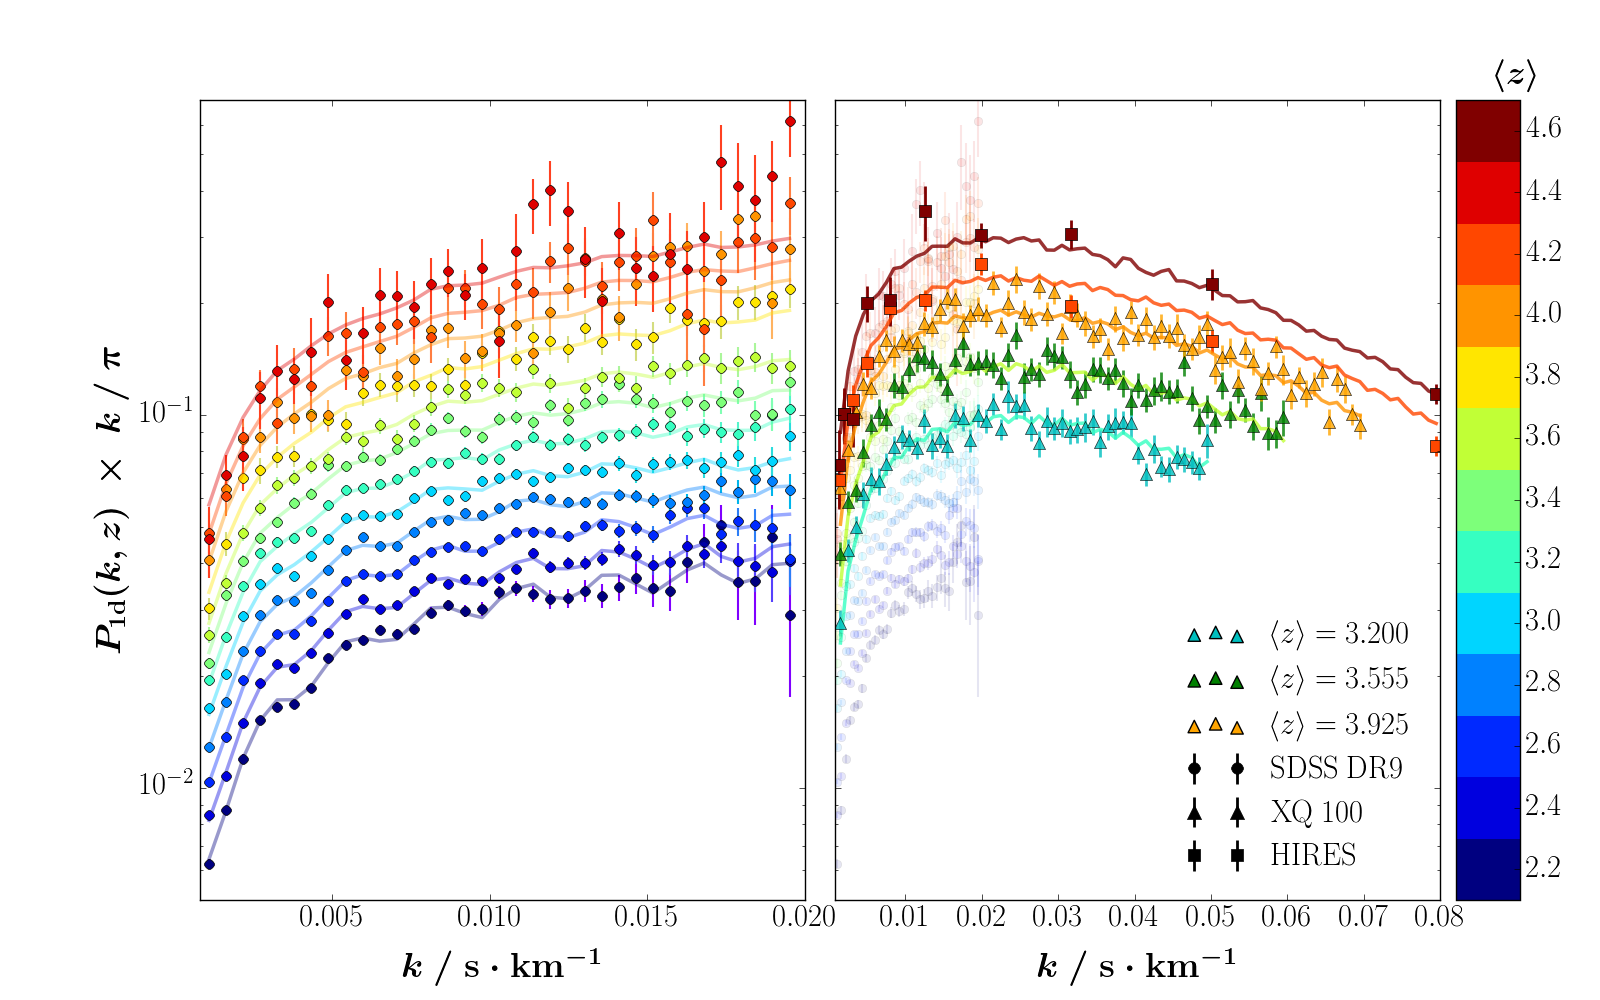
\includegraphics[width=0.9\columnwidth]{Data/Data_DR9_XQ_HR_fit.png}
\caption{\textbf{Left:} Dimensionless Ly-$\alpha$ power spectrum measured with SDSS DR9 (BOSS). The solid lines are the best-fit models derived with our likelihood analysis in each (color-coded) redshift bin. \textbf{Right:} Ly-$\alpha$ power spectrum measured with the XQ-100 (triangles) and MIKE+HIRES (square) quasar samples, overlayed with the BOSS DR9 sample (circles) for comparison.}
\label{fig:data_lya}
\end{center}
\end{figure}

The Ly-$\alpha$ flux power spectrum obtained with our simulations for ourcosmological models are fitted with the data set I detailed in Sec.~\ref{sec:pfdata}. In \cite{Palanque2015a, Palanque2015b, Baur16}, we used the Ly-$\alpha$ power spectrum in the 12 redshift bins of the SDSS DR9 sample set, which I hereafter label `BOSS' or `SDSS' data set, and re-transcribed in the left panel of Fig.~\ref{fig:data_lya}. In \cite{Yeche17, Baur17, Armengaud_FDM}, we also make use of higher-resolution data sets. Specifically, I include the Ly-$\alpha$ power spectrum measured at the $\langle z \rangle = 3.925, 3.555$ and $3.200$ redshifts using the 100 medium-resolution quasar spectra from the XShooter spectrograph (which I label `XQ-100' or `XQ' in all subsequent discussions), and/or the handful of high-resolution quasars from the MIKE and HIRES spectrographs (label `MIKE+HIRES' or `HR' in all that follows) limitted to the $\langle z \rangle = 4.2$ and $4.6$ redshift bins since we lack snapshot outputs for the $\langle z \rangle = 5.0$ and $5.4$. These two additional data sets are displayed in the right panel of Fig.~\ref{fig:data_lya}. \\

\begin{figure}
\begin{center}
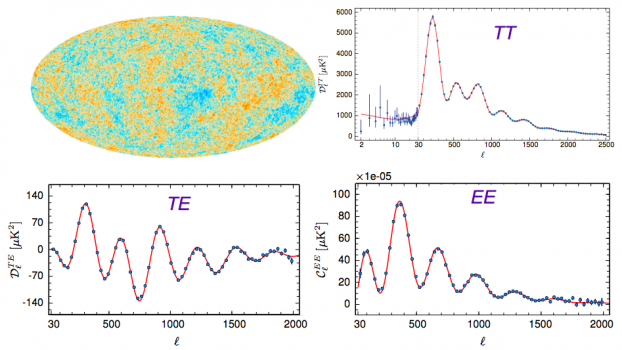
\includegraphics[width=0.9\columnwidth]{Data/data_cmb.png}
\caption{Mollweide projection of the CMB temperature anisotropies measured with the Planck spacecraft (top left). Clockwise from top right: temperature, E mode polarization auto-correlation and their cross correlation power spectra, with the best fit model in solid red. Credit: Figure from \url{http://www.insu.cnrs.fr/images/10841}, adapted from \cite{Planck2015}.}
\label{fig:data_cmb}
\end{center}
\end{figure}

Ly-$\alpha$ forests poorly probe certain cosmological parameters such as the expansion rate $H_0$. We therefore also include the $\chi^2$ derived from Planck data on the CMB. We use 
 the central values and  covariance matrices available in the official 
 Planck repositories\footnote{\tt http://wiki.cosmos.esa.int/planckpla2015/index.php/Main\_Page}  
for  the cosmological parameters  ($\sigma_8$, $n_s$, $\Omega_m$,  $H_0$, $n_{\rm run}$). Doing so also enables to aleviate the degeneracies between parameters, such as $\Omega_m$ and $\sigma_8$ with $\sum m_\nu$ for instance. For each parameter, we assume a Gaussian CMB likelihood with asymmetric $1\sigma$ errors that we estimate on either side of the central value from the $1\sigma$ lower and upper limits, thus accounting for asymmetric contours. We validated this strategy in \cite{Palanque2015a}, where we showed that it gave similar results to a Markov-Chain Monte-Carlo approach based on the full likelihood. I refer to the CMB temperature auto-correlation power spectrum fitted by Planck as `Planck TT', the low-multipole HFI-based polarization data up to $\ell \leqslant 29$ as `lowP', and the $\ell \geqslant 30$ polarization cross and auto-correlation as `TE' and `EE'. These angular power spectra are displayed in Fig.~\ref{fig:data_cmb}. \\


\begin{figure}
\begin{center}
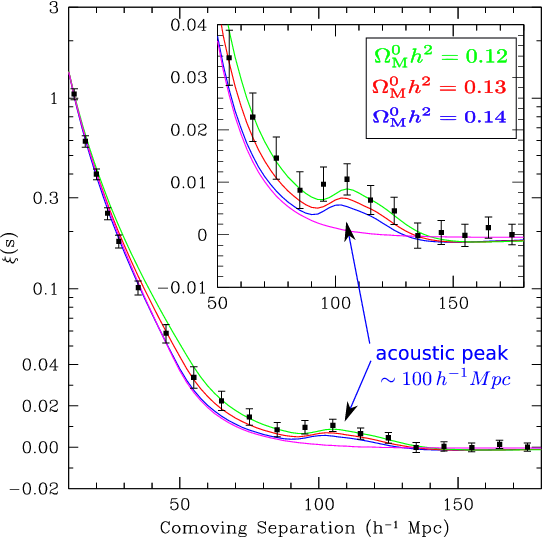
\includegraphics[width=0.5\columnwidth]{Data/BAO_spectrum.png}
\caption{The redshift-space correlation function of the SDSS Luminous Red Galaxy (LRG) sample from \cite{EisensteinBAO}. The magenta line shows a pure CDM model ($\omega_m = 0.105$) which lacks the acoustic peak. The green, red and blue lines are models with $\omega_b = 0.024$ for the baryon density and, respectively, $\omega_m = 0.12, 0.13$ and $0.14$. The BAO peak is visible at $\sim 100~h^{-1}\mathrm{Mpc}$. Credit: Figure from \cite{BAOplot}, adapted from \cite{EisensteinBAO}.}
\label{fig:data_bao}
\end{center}
\end{figure}

Finally, the Baryon Acoustic Oscillations (BAO) scale, illustrated in Fig.~\ref{fig:data_bao}, is also impacted by cosmological parameters. We therefore make use of measurements of the BAO scale by 6dFGS \cite{6dFGS}, the main galaxy sample of SDSS \cite{SDSSmainGalaxy}, the BOSS LOW-Z sample \cite{LOWZ-CMASS} and the CMASS DR11 sample \cite{LOWZ-CMASS}. This data set is labeled `BAO' herein.

\clearpage